\section{Introduzione}

\subsection{Obiettivo}

Vogliamo misurare il rate per unità di superficie orizzontale
dei raggi cosmici che passano nel laboratorio.

\subsection{Apparato}

La parte principale dell'apparato sono 6 lastre di scintillatore plastico
posizionate orizzontalmente e allineate verticalmente,
che non possiamo spostare,
collegate a tubi fotomoltiplicatori (vedi \autoref{fig:apparato}).

Disponiamo anche di un piccolo scintillatore mobile (il <<miniscint>>) (\autoref{fig:miniscint})
che può essere appoggiato sulle lastre principali.

\begin{figure}[H]
	\center
	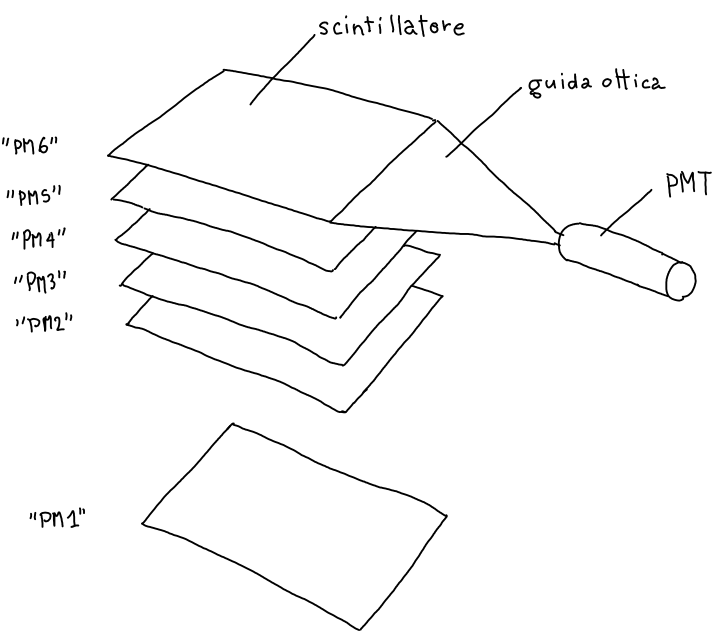
\includegraphics[width=\textwidth]{apparato}
	\caption{\label{fig:apparato}
	Apparato di misura.
	La struttura portante non è disegnata.
	La guida ottica e il tubo fotomoltiplicatore (PMT) sono disegnati solo per il PM6.}
\end{figure}

\begin{figure}[H]
	\center
	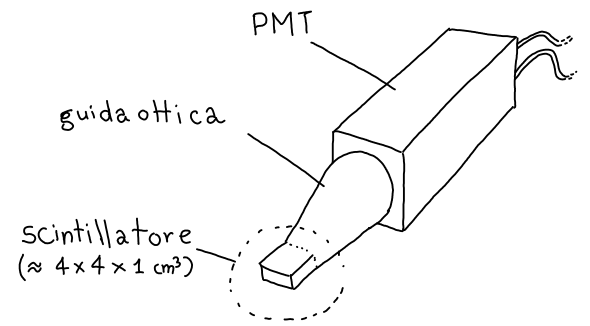
\includegraphics[width=23em]{miniscint}
	\caption{\label{fig:miniscint}
	Piccolo scintillatore mobile, che chiamiamo \emph{miniscint}.}
\end{figure}

